\documentclass[]{scrartcl}
\usepackage{lmodern}
\usepackage{amssymb,amsmath}
\usepackage{ifxetex,ifluatex}
\usepackage{fixltx2e} % provides \textsubscript
\ifnum 0\ifxetex 1\fi\ifluatex 1\fi=0 % if pdftex
  \usepackage[T1]{fontenc}
  \usepackage[utf8]{inputenc}
\else % if luatex or xelatex
  \ifxetex
    \usepackage{mathspec}
  \else
    \usepackage{fontspec}
  \fi
  \defaultfontfeatures{Ligatures=TeX,Scale=MatchLowercase}
\fi
% use upquote if available, for straight quotes in verbatim environments
\IfFileExists{upquote.sty}{\usepackage{upquote}}{}
% use microtype if available
\IfFileExists{microtype.sty}{%
\usepackage{microtype}
\UseMicrotypeSet[protrusion]{basicmath} % disable protrusion for tt fonts
}{}
\usepackage{hyperref}
\hypersetup{unicode=true,
            pdftitle={Angabe},
            pdfauthor={Team\ldots{}},
            pdfborder={0 0 0},
            breaklinks=true}
\urlstyle{same}  % don't use monospace font for urls
\IfFileExists{parskip.sty}{%
\usepackage{parskip}
}{% else
\setlength{\parindent}{0pt}
\setlength{\parskip}{6pt plus 2pt minus 1pt}
}
\setlength{\emergencystretch}{3em}  % prevent overfull lines
\providecommand{\tightlist}{%
  \setlength{\itemsep}{0pt}\setlength{\parskip}{0pt}}
\setcounter{secnumdepth}{5}
% Redefines (sub)paragraphs to behave more like sections
\ifx\paragraph\undefined\else
\let\oldparagraph\paragraph
\renewcommand{\paragraph}[1]{\oldparagraph{#1}\mbox{}}
\fi
\ifx\subparagraph\undefined\else
\let\oldsubparagraph\subparagraph
\renewcommand{\subparagraph}[1]{\oldsubparagraph{#1}\mbox{}}
\fi

\usepackage{graphicx}
\usepackage{array}
\usepackage{ragged2e}
\usepackage[section]{placeins}
\makeatletter
\AtBeginDocument{%
  \expandafter\renewcommand\expandafter\subsection\expandafter{%
    \expandafter\@fb@secFB\subsection
  }%
}
\makeatother
 
\title{Angabe 1}
\providecommand{\subtitle}[1]{}
\subtitle{Untertitel}
\author{Daniel Graf, Dimitrie Diez, Arne Schöntag, Peter Müller}
\date{}

\begin{document}
\maketitle


\tableofcontents

\section{Einführung}

% Problem -> Motivation

\section{Messexperiment}

Das Messexperiment wurde am $05.04.2017$ im Lichthof der Hochschule München (Lothstraße 64) durchgeführt. Es nahmen $22$ Probanden im Alter von $20-29$ Jahren teil. Das Experiment bestand aus drei Teilen. 

Zunächst wurde die Wunschgeschwindigkeit in der Ebene gemessen. Hierfür ging jeder Proband eine markierte Strecke von $27,3m$ ab und stoppte die hierfür benötigte Zeit. Anschließend wurde dieser Vorgang zweimal wiederholt und die entsprechende Rundennummer vermerkt. Im zweiten Teil erfolgte die Messung der benötigten Zeit für einen Treppenaufstieg. Die Treppenlänge betrug $9m$. Jeder Proband führte den Vorgang dreimal durch und vermerkte die benötigte Zeit und die entsprechende Rundennummer. Analog hierzu wurde im dritten Teil des Experiments die Zeit beim Treppenabstieg gemessen. 

Neben den gemessenen Zeiten in jeder Runde, dem Alter und der Körpergröße ist auch das Geschlecht jedes Probanden bekannt. Weitere Informationen sind in der beiliegenden Versuchsbeschreibung "Choreographie\_Treppengeschwindigkeit\_2017" aufgeführt. In den folgenden Kapiteln erfolgt die Auswertung der ermittelten Messwerte.

\section{Überprüfung auf Normalverteilung}
\section{Modell}
\section{Lineare Regression}
\subsection{Prüfung auf eine Abhängigkeit}
\subsection{Mehrere Abhängigkeiten}
\subsection{Konditionierung}

\section{Ergebnisse}
\section{Ermitteltes Modell}

\section{Vergleich mit Daten aus 2012}
\subsection{Überprüfung auf Normalverteilung}
\subsection{Lineare Regression}
\subsection{Vergleich}

\section{Verbund von alten und neuen Daten}
Unter der Annahme, dass die Bedingungen zum Zeitpunkt des Messexperiments im Jahr 2012 ähnlich waren wie im Jahr 2017, kann man die erfassten Daten aus beiden Experimenten zu einem gemeinsamen Datensatz zusammenfassen. Dies kann von Vorteil sein, da es sich insgesamt um mehr Teilnehmer handelt und so die Aussagekraft der Berechnungen erhöht wird. Es ist jedoch zu bedenken, dass folgende Faktoren die Aussagekraft verringern können. Zum einen hat eine Abweichung der Messbedingungen von 2012 zum Jahr 2017 direkten Einfluss auf die Messergebnisse. Zum Beispiel hat die Treppenhöhe einen enormen Einfluss auf die Treppengeschwindigkeit. Darüber hinaus ist zu bemerken, dass unter Umständen in beiden Experimenten ein und dieselbe Person teilgenommen hat und unter unterschiedlicher Probanden ID geführt wird. Dies kann zum Beispiel bedeuten, dass es in den Datensätzen zwei Personen mit der gleichen Körpergröße gibt. Diese Doppelerfassung einer Person hat zur Folge, dass die betreffende Person die Auswertung mit mehr Gewicht beeinflusst. 
Für die weitere Auswertung wird angenommen, dass die Messbedingungen beider Experimente annähernd gleich sind und es durch die lange Zeit zwischen den beiden Experimenten keine Doppelfassungen von Personen gibt. Der Fokus liegt vor allem auf der Analyse der linearen Regression. 

Es ist zu beachten, dass für alle Abbildungen und Gleichungen die Geschwindigkeiten in $\frac{m}{s}$ und die Größe in $cm$ angegeben sind. Die Rundenzahl hat keine Einheit bzw. die Einheit $1$.
\subsection{Prüfung auf eine einfache Abhängigkeit}
Zunächst wird die Abhängigkeit der Treppengeschwindigkeit von einem Parameter untersucht. Dabei werden jeweils die Parameter Wunschgeschwindigkeit in der Ebene, Größe und Rundenzahl beleuchtet. Mittels linearer Regression werden folgende Gleichungen ermittelt: 
\begin{align*}
v_{auf}(v_{ebene}) = \beta _0 + \beta _1 v_{ebene} \\
v_{ab}(v_{ebene}) = \beta _0 + \beta _1 v_{ebene} \\
v_{auf}(groesse) = \beta _0 + \beta _1 groesse \\
v_{ab}(groesse) = \beta _0 + \beta _1 groesse \\
v_{auf}(runde) = \beta _0 + \beta _1 runde \\
v_{ab}(runde) = \beta _0 + \beta _1 runde
\end{align*}
\subsubsection{Wunschgeschwindigkeit in der Ebene}
Aus der Erstellung eines linearen Regressionsmodells der Treppengeschwindigkeit in Abhängigkeit von der Wunschgeschwindigkeit in der Ebene ergeben sich folgende Gleichungen:
\begin{equation}
v_{auf}(v_{ebene}) = -0.908778 + 1.183660 v_{ebene}
\label{eq:2012_2017_AufEbene_MA}
\end{equation}
\begin{equation}
v_{ab}(v_{ebene}) = -0.0207308+0.724824 v_{ebene}
\label{eq:2012_2017_AbEbene_MA}
\end{equation}
Die zugehörigen Abbildungen \ref{fig:2012_und_2017_MA_auf_ebene} und \ref{fig:2012_und_2017_MA_ab_ebene} zeigen, dass die Regressionsgerade in beiden Fällen eine positive Steigung aufweist. Die Steigung der Treppengeschwindigkeit beim Aufwärtsgehen der Treppen (Gleichung \ref{eq:2012_2017_AufEbene_MA}) ist höher als im Jahr 2017 (Gleichungen \ref{eq:auf2017-ebene} und \ref{eq:ab2017-ebene}). Auch beim Abwärtsgehen ist die Regressionsgerade deutlich steiler als im Jahr 2017. In den Abbildungen \ref{fig:2012_und_2017_MA_auf_ebene} und \ref{fig:2012_und_2017_MA_ab_ebene} wird gezeigt, dass einige wenige Probanden deutlich schneller sind als der Rest. Die Entfernung der Ausreißer aus der Analyse wie in Abbildungen \ref{fig:2012_und_2017_OA_auf_ebene} und \ref{fig:2012_und_2017_OA_ab_ebene} zu sehen ist, ergibt folgende Gleichungen: 
\begin{equation}
v_{auf}'(v_{ebene}) = 0.44619 +0.232299 v_{ebene}
\label{eq:2012_2017_AufEbene_OA}
\end{equation}
\begin{equation}
v_{ab}'(v_{ebene}) = 0.759833 +0.191744 v_{ebene}
\label{eq:2012_2017_AbEbene_OA}
\end{equation}
Die Steigung der Regressionsgeraden ist deutlich geringer, wenn man die Ausreißer entfernt. 
Für die Plausibilisierung wird die Nullhypothese $H_0: \beta_1 = 0$ aufgestellt. Das Signifikanzniveau $\alpha= 0.05$. In beiden Fällen liegt Signifikanz vor, da der P-Wert $p<\alpha$ ist.

\begin{figure}[htpb]
\centering
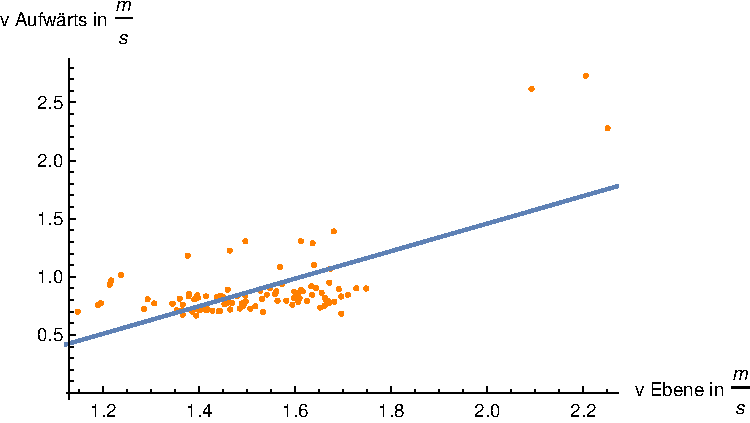
\includegraphics[width=0.7\textwidth]{abbildungen/regression/2012_2017_verbund/auf-ebene.pdf}
\justify \ \\
Ergebnisse der Plausibilisierung für den Aufstieg:
\[\begin{array}{l|llll}
 \text{} & \text{Estimate} & \text{Standard Error} & \text{t-Statistic} & \text{P-Value} \\
\hline
 1 & 0.506746 & 0.0900029 & 5.63033 & \text{2.603647901106944$\grave{ }$*${}^{\wedge}$-6} \\
 \text{vEbene} & 0.168071 & 0.0588553 & 2.85567 & 0.00727064 \\
\end{array}\]


\caption{Abhängigkeit der Wunschgeschwindigkeit in der Ebene und der Treppengeschwindigkeit aufwärts. Messdaten (orange) mit ermittelter Regressionsgeraden (blau)}
\label{fig:2012_und_2017_MA_auf_ebene}
\end{figure}

\begin{figure}[htpb]
\centering
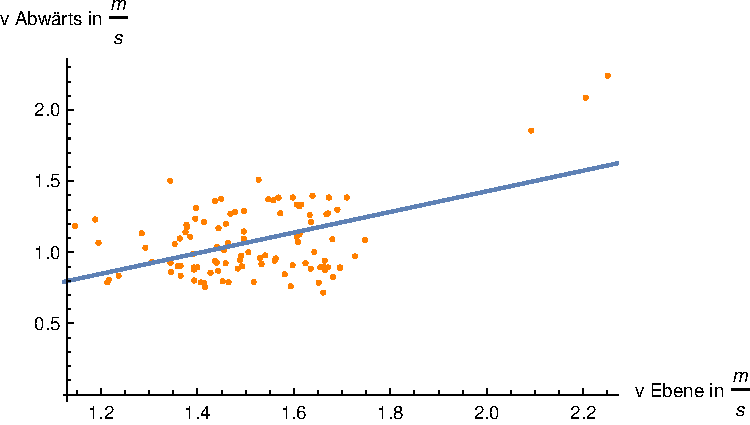
\includegraphics[width=0.7\textwidth]{abbildungen/regression/2012_2017_verbund/ab-ebene.pdf}
\justify \ \\
Ergebnisse der Plausibilisierung für den Abstieg:
\[\begin{array}{l|llll}
 \text{} & \text{Estimate} & \text{Standard Error} & \text{t-Statistic} & \text{P-Value} \\
\hline
 1 & 0.440848 & 0.213068 & 2.06904 & 0.0428577 \\
 \text{vEbene} & 0.478525 & 0.142985 & 3.34668 & 0.00141579 \\
\end{array}\]


\caption{Abhängigkeit der Wunschgeschwindigkeit in der Ebene und der Treppengeschwindigkeit abwärts. Messdaten (orange) mit ermittelter Regressionsgeraden (blau)}
\label{fig:2012_und_2017_MA_ab_ebene}
\end{figure}

\begin{figure}[htpb]
\centering
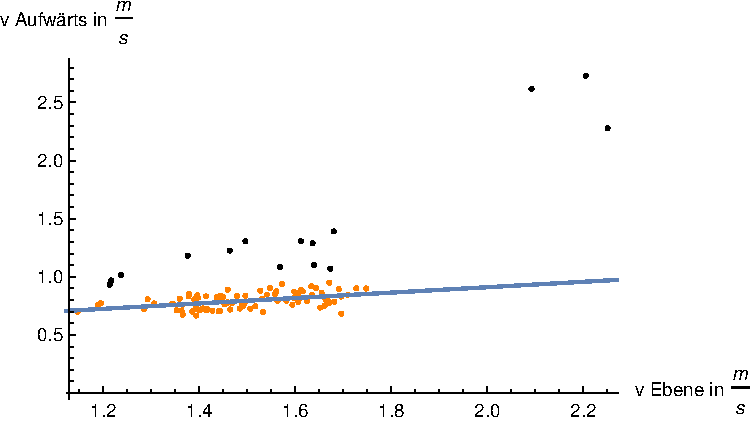
\includegraphics[width=0.7\textwidth]{abbildungen/regression/2012_2017_verbund/ohneausreisser/auf-ebene.pdf}
\justify \ \\
Ergebnisse der Plausibilisierung für den Aufstieg:
\[\begin{array}{l|llll}
 \text{} & \text{Estimate} & \text{Standard Error} & \text{t-Statistic} & \text{P-Value} \\
\hline
 1 & 0.506746 & 0.0900029 & 5.63033 & \text{2.603647901106944$\grave{ }$*${}^{\wedge}$-6} \\
 \text{vEbene} & 0.168071 & 0.0588553 & 2.85567 & 0.00727064 \\
\end{array}\]


\caption{Abhängigkeit der Wunschgeschwindigkeit in der Ebene und der Treppengeschwindigkeit aufwärts. Messdaten (orange) und Ausreißer (schwarz) mit ermittelter Regressionsgeraden (blau)}
\label{fig:2012_und_2017_OA_auf_ebene}
\end{figure}

\begin{figure}[htpb]
\centering
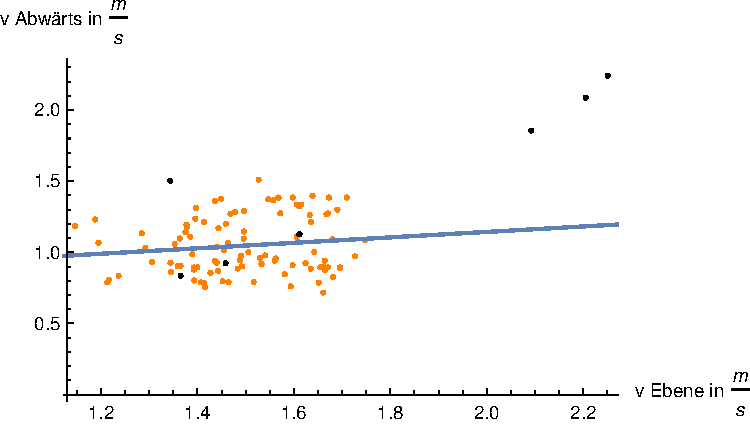
\includegraphics[width=0.7\textwidth]{abbildungen/regression/2012_2017_verbund/ohneausreisser/ab-ebene.pdf}
\justify \ \\
Ergebnisse der Plausibilisierung für den Abstieg:
\[\begin{array}{l|llll}
 \text{} & \text{Estimate} & \text{Standard Error} & \text{t-Statistic} & \text{P-Value} \\
\hline
 1 & 0.440848 & 0.213068 & 2.06904 & 0.0428577 \\
 \text{vEbene} & 0.478525 & 0.142985 & 3.34668 & 0.00141579 \\
\end{array}\]


\caption{Abhängigkeit der Wunschgeschwindigkeit in der Ebene und der Treppengeschwindigkeit abwärts. Messdaten (orange) und Ausreißer (schwarz) mit ermittelter Regressionsgeraden (blau)}
\label{fig:2012_und_2017_OA_ab_ebene}
\end{figure}













\subsubsection{Körpergröße}
Für die Abhängigkeit zu Körpergröße werden nur Daten ohne die zuvor genannten Ausreißer herangezogen. Da es beispielsweise Probanden gab, die gerannt sind, ist es nicht sinnvoll, diese in Beziehung zur Körpergröße zu setzen. Es wurde folgender Zusammenhang ermittelt:
\begin{equation}
v_{auf}(groesse) = 1.4018 -0.00342982 groesse
\label{eq:2012_2017_AufGroesse_MA}
\end{equation}
\begin{equation}
v_{ab}(groesse) = 1.85077 -0.0045234 groesse
\label{eq:2012_2017_AbGroesse_MA}
\end{equation}
Grafisch dargestellt wird dieser Zusammenhang in den Abbildungen \ref{fig:2012_und_2017_MA_auf_groesse} und \ref{fig:2012_und_2017_MA_ab_groesse}. In den darunterliegenden Tabellen sind die Ergebnisse der Plausibilisierungstests zu sehen. Beim Treppenaufstieg ist der P-Wert $p<\alpha$. Signifikanz liegt vor und die Nullhypothese wird abgelehnt. Die Körpergröße hat beim Aufstieg einen direkten Einfluss auf die Treppengeschwindigkeit. Beim Abstieg ist der P-Wert nur geringfügig größer als das Signifikanzniveau $\alpha$. Es ist also anzunehmen, dass die Körpergröße beim Abstieg keine Auswirkung auf die Treppengeschwindigkeit hat. Diese Erkenntnis ist plausibel, da beim Aufstieg die Beinlänge eine bedeutendere Rolle spielt als beim Abstieg. Interessant ist die  Tatsache, dass beide Regressionsgeraden eine negative Steigung haben. Je größer ein Proband, desto niedriger ist die Geschwindigkeit beim Treppensteigen.

\begin{figure}[htpb]
\centering
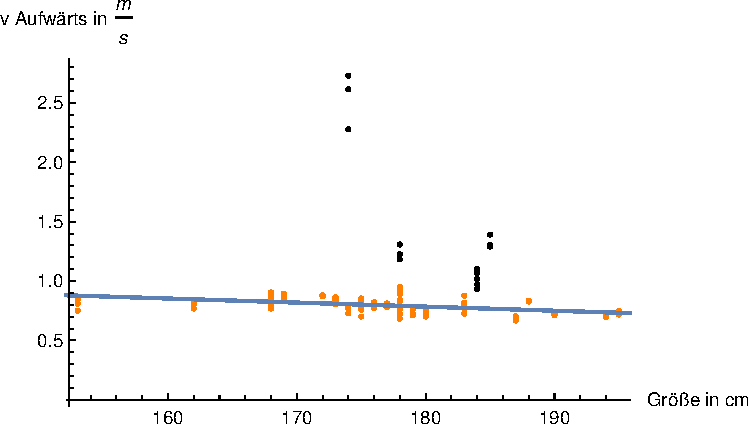
\includegraphics[width=0.7\textwidth]{abbildungen/regression/2012_2017_verbund/ohneausreisser/auf-groesse.pdf}
\justify \ \\
Ergebnisse der Plausibilisierung für den Aufstieg:
\[\begin{array}{l|llll}
 \text{} & \text{Estimate} & \text{Standard Error} & \text{t-Statistic} & \text{P-Value} \\
\hline
 1 & 1.42188 & 0.660147 & 2.15388 & 0.0335816 \\
 \text{gr{\" o}{\ss}e} & -0.00301832 & 0.0037105 & -0.813455 & 0.417834 \\
\end{array}\]


\caption{Abhängigkeit der Körpergröße und der Treppengeschwindigkeit aufwärts. Messdaten (orange) und Ausreißer (schwarz) mit ermittelter Regressionsgeraden (blau)}
\label{fig:2012_und_2017_MA_auf_groesse}
\end{figure}



\begin{figure}[htpb]
\centering
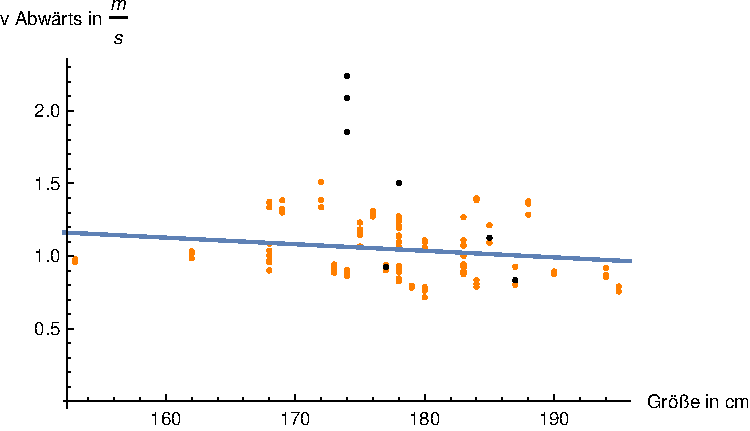
\includegraphics[width=0.7\textwidth]{abbildungen/regression/2012_2017_verbund/ohneausreisser/ab-groesse.pdf}
\justify \ \\
Ergebnisse der Plausibilisierung für den Abstieg:
\[\begin{array}{l|llll}
 \text{} & \text{Estimate} & \text{Standard Error} & \text{t-Statistic} & \text{P-Value} \\
\hline
 1 & 1.59558 & 0.582855 & 2.73753 & 0.00800578 \\
 \text{gr{\" o}{\ss}e} & -0.00253145 & 0.00328881 & -0.769715 & 0.444301 \\
\end{array}\]


\caption{Abhängigkeit der Körpergröße und der Treppengeschwindigkeit abwärts. Messdaten (orange) und Ausreißer (schwarz) mit ermittelter Regressionsgeraden (blau)}
\label{fig:2012_und_2017_MA_ab_groesse}
\end{figure}




















\subsubsection{Rundennummer}
Auch für die Abhängigkeit zur Rundennummer wurden die Ausreißer entfernt. Folgender Zusammenhang wurde ermittelt:
\begin{equation}
v_{auf}(runde) = 0.800529 -0.00319011 runde
\label{eq:2012_2017_AufRunde_MA}
\end{equation}
\begin{equation}
v_{ab}(runde) = 1.03894 + 0.00414082 runde
\label{eq:2012_2017_AbRunde_MA}
\end{equation}
Die grafische Darstellung für diesen Zusammenhang ist für den Treppenaufstieg in Abbildung \ref{fig:2012_und_2017_MA_auf_runde} und für den Treppenabstieg in Abbildung \ref{fig:2012_und_2017_MA_ab_runde} zu sehen. Die Abbildungen machen bereits deutlich, dass eine Abhängigkeit der Treppengeschwindigkeit von der Rundenzahl nicht plausibel ist. Die Ergebnisse der Plausibilitätsprüfung in den Tabellen jeweils unter den Abbildungen zeigen, dass der P-Wert in beiden Fällen deutlich über dem Signifikanzniveau $\alpha$ liegt. Die Nullhypothese wird angenommen, die Rundenzahl hat keinen Einfluss auf die Treppengeschwindigkeit.











\begin{figure}[htpb]
\centering
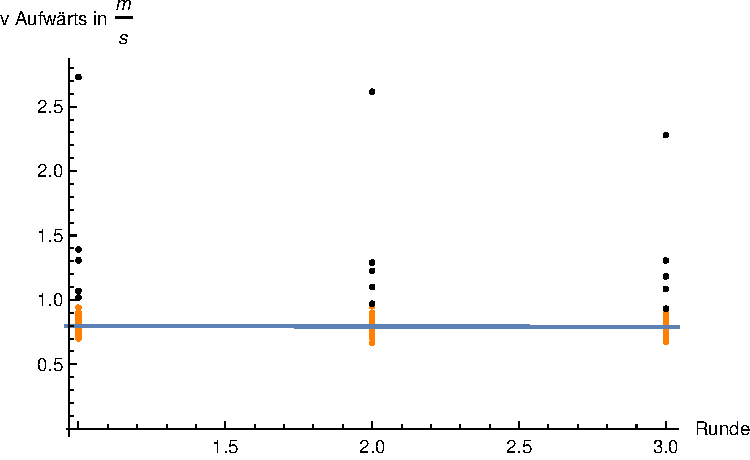
\includegraphics[width=0.7\textwidth]{abbildungen/regression/2012_2017_verbund/ohneausreisser/auf-runde.pdf}
\justify \ \\
Ergebnisse der Plausibilisierung für den Aufstieg:
\[\begin{array}{l|llll}
 \text{} & \text{Estimate} & \text{Standard Error} & \text{t-Statistic} & \text{P-Value} \\
\hline
 1 & 0.94804 & 0.2081 & 4.55569 & 0.0000551454 \\
 \text{runde} & -0.0241206 & 0.0963317 & -0.250391 & 0.80367 \\
\end{array}\]


\caption{Abhängigkeit der Runde und der Treppengeschwindigkeit aufwärts. Messdaten (orange) und Ausreißer (schwarz) mit ermittelter Regressionsgeraden (blau)}
\label{fig:2012_und_2017_MA_auf_runde}
\end{figure}



\begin{figure}[htpb]
\centering
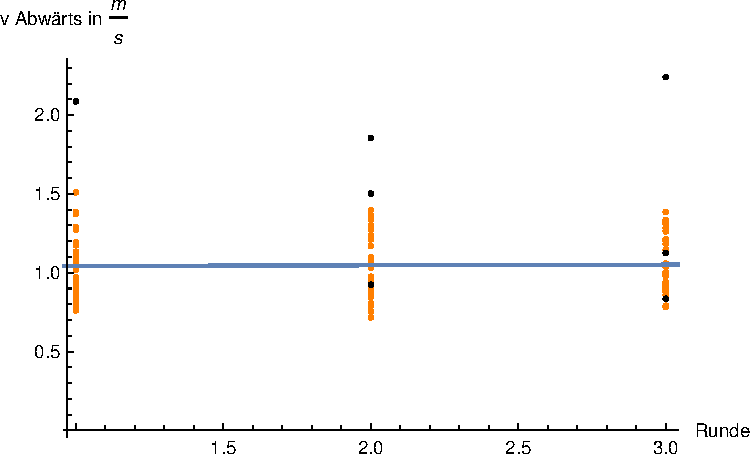
\includegraphics[width=0.7\textwidth]{abbildungen/regression/2012_2017_verbund/ohneausreisser/ab-runde.pdf}
\justify \ \\
Ergebnisse der Plausibilisierung für den Abstieg:
\[\begin{array}{l|llll}
 \text{} & \text{Estimate} & \text{Standard Error} & \text{t-Statistic} & \text{P-Value} \\
\hline
 1 & 0.859522 & 0.0289618 & 29.6777 & \text{6.817362585804904$\grave{ }$*${}^{\wedge}$-26} \\
 \text{runde} & 0.00475595 & 0.0134067 & 0.354744 & 0.724973 \\
\end{array}\]


\caption{Abhängigkeit der Runde und der Treppengeschwindigkeit abwärts. Messdaten (orange) und Ausreißer (schwarz) mit ermittelter Regressionsgeraden (blau)}
\label{fig:2012_und_2017_MA_ab_runde}
\end{figure}



\subsection{Prüfung auf mehrere Abhängigkeiten}
Es wird die Abhängigkeit der Treppengeschwindigkeit von mehreren Parametern untersucht. Mittels linearer Regression werden folgende Gleichungen ermittelt: 
\begin{align*}
v_{auf}(v_{ebene}, groesse) = \beta _0 + \beta _1 v_{ebene} + \beta _2 groesse \\
v_{ab}(v_{ebene}, groesse) = \beta _0 + \beta _1 v_{ebene} + \beta _2 groesse \\
v_{auf}(v_{ebene}, groesse, runde) = \beta _0 + \beta _1 v_{ebene} + \beta _2 groesse + \beta _3 runde \\
v_{ab}(v_{ebene}, groesse, runde) = \beta _0 + \beta _1 v_{ebene} + \beta _2 groesse + \beta _3 runde \\
\end{align*}
Auch hier werden die Ausreißer vor der Berechnung entfernt. In den Abbildungen sind die Ausreißer schwarz dargestellt. Analog zu den vorherigen Kapiteln wird eine Nullhypothese $H_0: \beta _1 = 0,\ \beta _2 = 0,\ \beta _3 = 0$ aufgestellt und eine Plausibilitätsprüfung durchgeführt. Das Signifikanzniveau $\alpha$ wird mit $0,05$ definiert.
\subsubsection{Lineare Regression mit zwei Parametern}
Bei der Erstellung eines linearen Regressionsmodells der Treppengeschwindigkeit in Abhängigkeit von Ebenengeschwindigkeit und Körpergröße ergibt sich folgender Zusammenhang:
\begin{equation}
v_{auf}(v_{ebene}, groesse) = 1.0165 -0.00294506 groesse+0.199894 v_{ebene}
\end{equation}
\begin{equation}
v_{ab}(v_{ebene}, groesse) = 1.55685 -0.00417799 groesse +0.155209 v_{ebene}
\end{equation}
Grafisch dargestellt ergibt dies eine Fläche wie in Abbildungen \ref{fig:2012_und_2017_OA_auf_ebene_groesse} und  \ref{fig:2012_und_2017_OA_ab_ebene_groesse} zu sehen ist. Die Plausibilitätsprüfung ergibt für den Aufstieg eine Abhängigkeit der Treppengeschwindigkeit von den Parametern Wunschgeschwindigkeit in der Ebene und der Größe. Für den Treppenabstieg wird die Nullhypothese angenommen, da der P-Wert über dem Signifikanzniveau liegt. Die Treppengeschwindigkeit beim Abstieg ist nicht von den Parameter Ebenengeschwindigkeit und Größe abhängig. 




\begin{figure}[htpb]
\centering
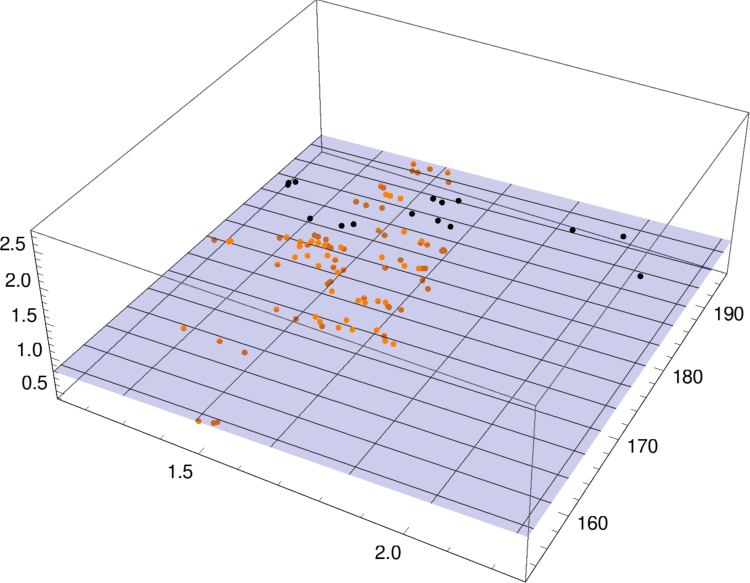
\includegraphics[width=0.7\textwidth]{abbildungen/regression/2012_2017_verbund/ohneausreisser/auf-ebene-groesse.pdf}
\justify \ \\
Ergebnisse der Plausibilisierung für den Aufstieg:
\[\begin{array}{l|llll}
 \text{} & \text{Estimate} & \text{Standard Error} & \text{t-Statistic} & \text{P-Value} \\
\hline
 1 & 1.0165 & 0.140132 & 7.25384 & \text{1.5820003769083974$\grave{ }$*${}^{\wedge}$-10} \\
 \text{vEbene} & 0.199894 & 0.0433176 & 4.61461 & 0.0000134806 \\
 \text{gr{\" o}{\ss}e} & -0.00294506 & 0.000643082 & -4.5796 & 0.0000154292 \\
\end{array}\]


\caption{Abhängigkeit der Ebenengeschwindigkeit, der Größe und der Treppengeschwindigkeit aufwärts. Messdaten (orange) und Ausreißer (schwarz) mit ermittelter Regressionsfläche (blau)}
\label{fig:2012_und_2017_OA_auf_ebene_groesse}
\end{figure}



\begin{figure}[htpb]
\centering
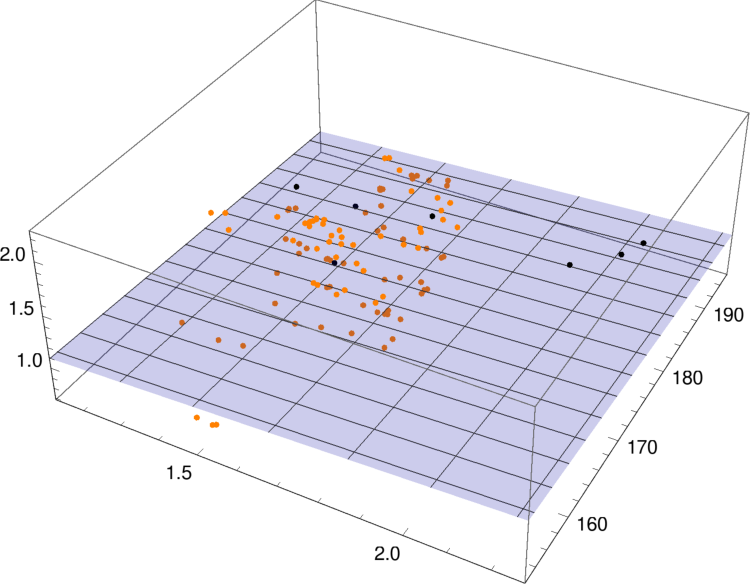
\includegraphics[width=0.7\textwidth]{abbildungen/regression/2012_2017_verbund/ohneausreisser/ab-ebene-groesse.pdf}
\justify \ \\
Ergebnisse der Plausibilisierung für den Abstieg:
\[\begin{array}{l|llll}
 \text{} & \text{Estimate} & \text{Standard Error} & \text{t-Statistic} & \text{P-Value} \\
\hline
 1 & 0.701775 & 0.543236 & 1.29184 & 0.199331 \\
 \text{vEbene} & 0.696676 & 0.127843 & 5.44946 & \text{3.523565756565165$\grave{ }$*${}^{\wedge}$-7} \\
 \text{gr{\" o}{\ss}e} & -0.00382545 & 0.00268911 & -1.42257 & 0.157912 \\
\end{array}\]


\caption{Abhängigkeit der Ebenengeschwindigkeit, der Größe und der Treppengeschwindigkeit abfwärts. Messdaten (orange) und Ausreißer (schwarz) mit ermittelter Regressionsfläche (blau)}
\label{fig:2012_und_2017_OA_ab_ebene_groesse}
\end{figure}









\subsubsection{Lineare Regression mit drei Parametern}
Bei der Erstellung eines linearen Regressionsmodells der Treppengeschwindigkeit in Bezug zu Ebenengeschwindigkeit, Körpergröße und Rundenzahl ergibt sich folgender Zusammenhang:
\begin{multline}
v_{auf}(v_{ebene}, groesse, runde) = \\ 
1.02175 -0.00294612 groesse -0.00220598 runde +0.199456 v_{ebene}
\end{multline}
\begin{multline}
v_{ab}(v_{ebene}, groesse, runde ) = \\ 
2.17485 -0.0057147 groesse+0.00132958 runde -0.0829226 v_{ebene}
\end{multline}
Eine sinnvolle grafische Abbildung dieses Zusammenhangs ist leider nicht möglich. 
Eine Plausibilitätsprüfung ergibt folgende Ergebnisse für den Aufstieg:
\[\begin{array}{l|llll}
 \text{} & \text{Estimate} & \text{Standard Error} & \text{t-Statistic} & \text{P-Value} \\
\hline
 1 & -1.06201 & 0.581909 & -1.82505 & 0.0709498 \\
 \text{runde} & -0.0035349 & 0.0291243 & -0.121373 & 0.903637 \\
 \text{vEbene} & 1.18933 & 0.136075 & 8.74028 & \text{5.287415408789427$\grave{ }$*${}^{\wedge}$-14} \\
 \text{gr{\" o}{\ss}e} & 0.000853656 & 0.00286026 & 0.298454 & 0.76597 \\
\end{array}\]


Vor allem im Bezug auf die Rundenzahl ergibt sich ein P-Wert deutlich höher als das Signifikanzniveau $\alpha$. Der P-Wert in Bezug auf die Ebenengeschwindigkeit und die Körpergröße liegt unter dem Signifikanzniveau.


Für den Abstieg ergibt sich folgende Plausibilitätsprüfung:
\[\begin{array}{l|llll}
 \text{} & \text{Estimate} & \text{Standard Error} & \text{t-Statistic} & \text{P-Value} \\
\hline
 1 & -0.893281 & 0.654301 & -1.36525 & 0.180888 \\
 \text{runde} & 0.0153806 & 0.0381571 & 0.403085 & 0.689337 \\
 \text{vEbene} & 1.27163 & 0.152749 & 8.32501 & \text{8.139962234647669$\grave{ }$*${}^{\wedge}$-10} \\
 \text{gr{\" o}{\ss}e} & -0.00100623 & 0.00306762 & -0.328015 & 0.744854 \\
\end{array}\]


Beim Treppenabstieg ist der P-Wert nur in Bezug auf die Körpergröße unter dem Signifiknazniveau $\alpha$.
















\section{Fazit}

\end{document}
